\documentclass[11pt]{article}

\usepackage[utf8x]{inputenc}
\usepackage[english]{babel}

\usepackage{amssymb}
\usepackage{amsmath} 
\usepackage{url}

\usepackage[toc,page]{appendix}

\usepackage{float}

\makeatletter
\newcommand*{\centerfloat}{
  \parindent \z@
  \leftskip \z@ \@plus 1fil \@minus \textwidth
  \rightskip\leftskip
  \parfillskip \z@skip}
\makeatother

\usepackage[pdftex]{graphicx} % za slike
\selectlanguage{english}

\title{\textbf{Robustness of persistence diagrams}}
\author{O\v zbolt Menegatti\\
		Anej Placer\\
		Jurij Slabanja}
\date{}
\begin{document}

\maketitle

\section{Project goal}

The goal of this project was to demonstrate the robustness of persistence diagrams of the Vietoris-Rips complex on a specific example.

\subsection{Vietoris-Rips}
Vietoris-Rips complex is very similar to Čech complex, but here we don't operate with virtual spheres. The distances between pairs of points are used instead. In Vietoris-Rips complex a simplex is part of the complex only if the diameter of the simplex is smaller or equal to $2\delta$ (maximal distance between two points). The difference from the Čech complex is easily observed if we consider vertexes from the equilateral triangle, while taking about half of the length of one side as can be seen in the Image~\ref{fig:vrdiag}. Čech complex would return an empty triangle, while Vietoris-Rips generates a full 2-simplex.\cite{Zomorodian2010263}

\begin{figure}[!htb]
    \centering
    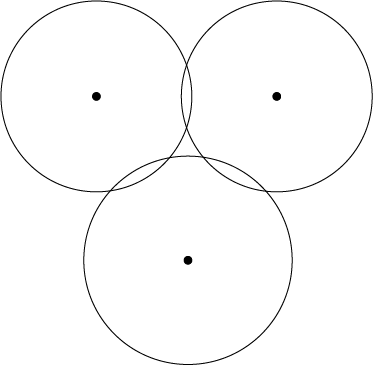
\includegraphics[width=0.4\textwidth]{vrdiag.png}
    \caption{The Vietoris-Rips complex generates a full triangle, whereas the Čech complex an empty one.}
    \label{fig:vrdiag}
\end{figure}

The Vietoris-Rips complex can be seen as a Čech complex in which the added complexes have all the faces included in Čech complex. It follows that the Čech complex is a subset of Vietoris-Rips complex. Of course if this is the case, both complexes must have the same parameter $\delta$. It's important to note that the Vietoris-Rips complex, similar to Čech complex, also has problems with high dimensional simplexes.

\subsection{Persistence}

Homology groups are one of the main concepts of algebraic topology. The topology is represented by the \emph{Betti numbers}, which represent the rank of the homology groups. Homology of degree 0 represents a connectedness of data (how many connected components are there), homology of degree 1 detects holes and tunnels, homology of degree 2 detects voids etc. In this assignment we limited our research to the first three important groups.

The connectedness of discrete points is represented with complexes. It depends on certain parameters like radius around the points, which tells us which points are interconnected. The connectedness therefore can't be defined universally.

This problem is solved by the concept of \emph{persistence}. The idea of persistence is, that by increasing the radius around the point, the complexes and homology groups also change. That however tells us which topology \emph{persists} through the changes.

In Image~\ref{homo} it can be observed that by increasing the radius, the graph becomes more connected. The lines in the diagram represent the ``life span'' of a topological feature. At some $\delta$ the number of crossed lines represents the Betti number for a specific degree. \cite{persist}

\begin{figure}[htb]
    \centering
    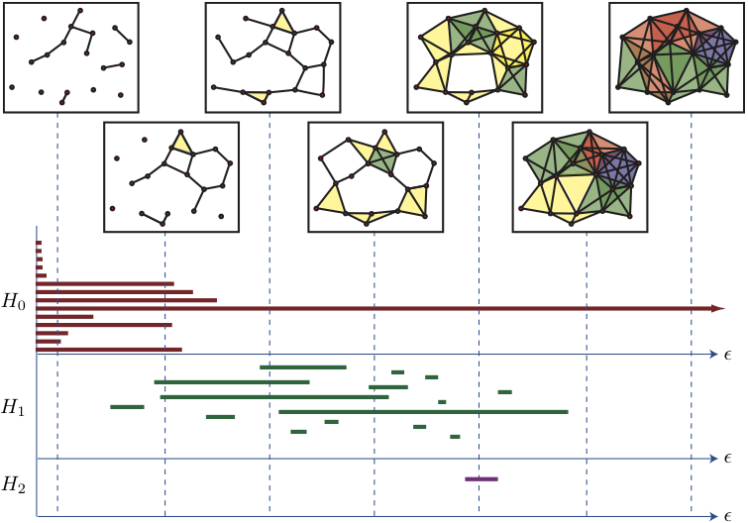
\includegraphics[width=0.8\textwidth]{homo.png}
    \caption{Persistence and the barcode diagram.}
    \label{homo}
\end{figure}

If we look at the second crossing, there are 6 connected components and two holes. In the assignment we filtered out all the entries that have the length of the line zero (is born and dies at the same delta).

Another way of using the persistence diagram is to plot the \emph{birth} and \emph{death} times of connected components (seen as lines in barcode diagram). Since each feature is represented by a $z = (birth, death)$ pair, we can plot this as points in a plane where the x-axis represents the birth of a feature and the y-axis it's death. Small features will have death times close to their birth times, which means they will be closer to the diagonal. The points near the diagonal can be looked at as \emph{topological noise} while those further away as \emph{topological signals}.


\section{Approach}

The data on which the robustness of persistence diagrams was to be demonstrated was the set of points \emph{S}. Then the largest distance \emph{R} between any two points in the data set \emph{S} was found and was divided into parts of increasing size: $0 = r_0 < r_1 < r_2 < ... < r_n = R$. For every \emph{r} the Vietoris-Rips complexes $V_i = V_ri(S), i = 0,...,n$ were constructed\footnote{$V_0$ represents a point cloud and $V_n$ is a fully connected graph.}. This represented a \emph{filtration} $V_0 \leq V_1 \leq ... \leq V_n$. Next the persistence diagram of the filtration in dimensions 0, 1 and 2 were computed. Finally the whole process was repeated many times on shaken up datasets, which were obtained by adding a small error term $\epsilon < R/100$ to the coordinates of each point in S.

We compared the persistence diagrams of the original and shaken datasets by plotting them on a single persistence diagram and attempted to connect disticnt features with a line. This way we could see how some feature moved around when we shook the dataset. The diagrams were also compared using bottleneck distance to numerically determine how similar the the persistence diagrams for the shaken datasets were to the original. The bottleneck distance measures how much we have to move the points in the shaken up persistence diagram to match the points from the original one. We also plotted the barcode diagrams for the obtained persistence diagrams.

This approach was performed on three datasets two large ones with 10000 points and a smaller one with 1000 points. Unfortunately due to the computational intensity required we only managed to calculate the bottleneck distance for the smaller dataset. With the other two we had to filter out so many points, to be able to compute the distance in a reasonable amount of time, that the results would have been largly meaningless. 

C++, Qt framework\cite{qt} and the topological computation library Dyonisus\cite{dionysus} were used to compute Vietoris-Rips complexes, while the diagrams were generated using Python\cite{python}.

\section{Results}

The persistence and barcode diagrams of the obtained results of all three datasets are shown in Appendix~\ref{appdix}. Each diagram is a composite of the original and shaken datasets. For example Figure~\ref{data1_pers} is a composite of the persistence diagram of the original dataset and the persistence diagrams of all the shaken dataset 1. Individual generators are connected with lines, so we can see how they move as we shake the dataset. For the most part it seems they are indeed constrained in small groups as one would expect. Sometimes though points on the diagram appear to jump out of their local group. We believe this is due to simple error and we go more into detail about this in Section~\ref{probs}.

The bottleneck distances were only calculated for the smaller dataset (dataset 2). The max distance for it was 7.5, hence the points in the shaken datasets were moved at most for $\epsilon = 0.075$. The results are shown in Table~\ref{tab:bottle_dist}. 

\begin{table}[H]
	\begin{tabular}{llllllllll}
		& O & S1 & S2 & S3 & S4 & S5 & S6 & S7 & S8 \\
		\hline
		O & 0.000 & 0.122 & 0.117 & 0.129 & 0.178 & 0.089 & 0.100 & 0.170 & 0.129 \\
		\\
		\\
		& S9 & S10 & S11 & S12 & S13 & S14 & S15 & S16 & avg \\
		\hline
		O& 0.122 & 0.130 & 0.113 & 0.107 & 0.128 & 0.125 & 0.120 & 0.434 & 0.154\\
	\end{tabular}
	\caption{Bottleneck distances between the persistence diagrams of the original \emph{O} and shaken \emph{S} datasets}
	\label{tab:bottle_dist}
\end{table}

\section{\label{probs}Problems}

We had some smaller problems, which were mostly solved by some compromises:

\begin{enumerate}
\item the datasets were too large, so we couldn't use the largest distance between two points, or the generation of Vietoris-Rips complex would have taken too long, so we used an arbitrarily chosen value smaller than the largest distance. 

\item when displaying the persistance diagrams some homology generators seem to jump out of their local group. This is probably best shown on the persistence diagram for dataset 2, where we have quite a few longer lines connecting ``individual'' generator groups. This is only a visual glitch since we don't know exactly which generators belong together after we shake the datasets and we make some assumptions based on which cycles the generators belong to. This does not impact the bottleneck distance results. 
\end{enumerate}

\section{Work distribution}

\subsection{Ožbolt}
Reading and formating of data, bottleneck distance, testing.

\subsection{Anej}
Vietoris-Rips, generation of diagrams.

\subsection{Jurij}
Project framework setup, dataset shaking, testing.

\newpage

\bibliographystyle{plain}
\bibliography{report-bib}

\newpage

\appendix
\appendixpage
\section{\label{appdix}Persistence and barcode diagrams}
For all the diagrams the red colour represents homology generators for dimension 0, the green are generators for dimension 1, and the blue represent dimension 2.
\begin{figure}[H]
   \centerfloat
   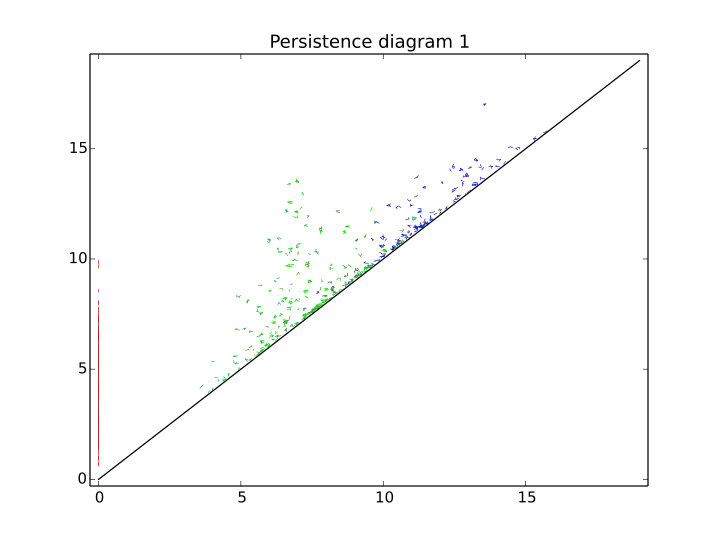
\includegraphics[width=1.2\textwidth]{data1_d18_pers.png}
   \caption{Persistance diagram for original and shaken dataset 1}
   \label{data1_pers}
\end{figure}

\begin{figure}[H]
   \centerfloat
   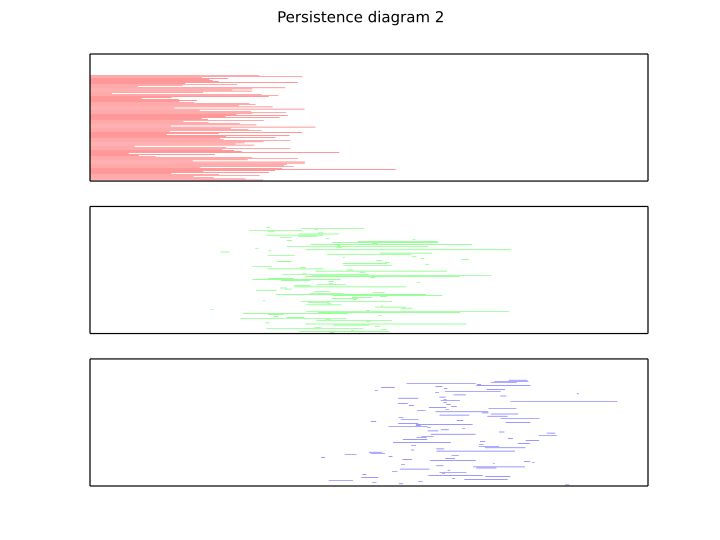
\includegraphics[width=1.2\textwidth]{data1_d18_bar.png}
   \caption{Barcode diagram for original and shaken dataset 1}
   \label{data1_bar}
\end{figure}

\begin{figure}[H]
   \centerfloat
   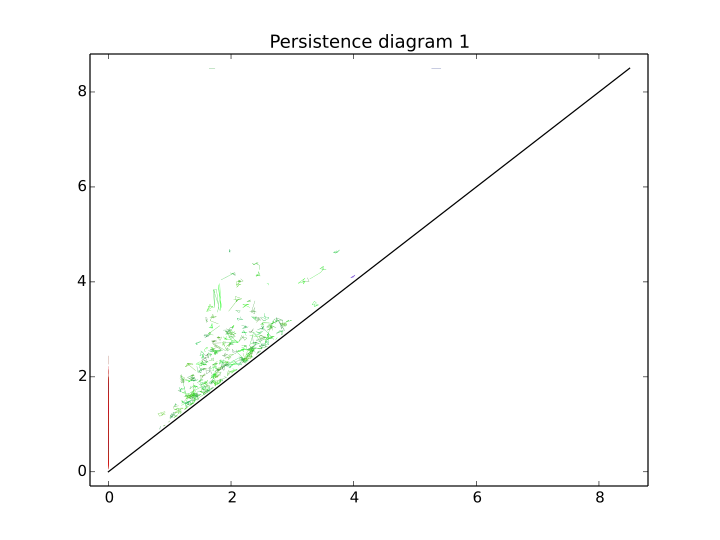
\includegraphics[width=1.2\textwidth]{data2_d7_5_pers.png}
   \caption{Persistance diagram for original and shaken dataset 2}
   \label{data2_pers}
\end{figure}

\begin{figure}[H]
   \centerfloat
   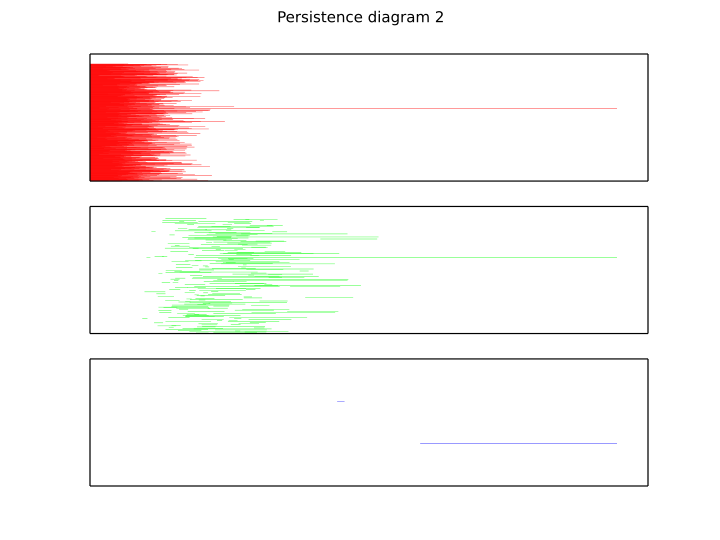
\includegraphics[width=1.2\textwidth]{data2_d7_5_bar.png}
   \caption{Barcode diagram for original and shaken dataset 2}
   \label{data2_bar}
\end{figure}

\begin{figure}[H]
   \centerfloat
   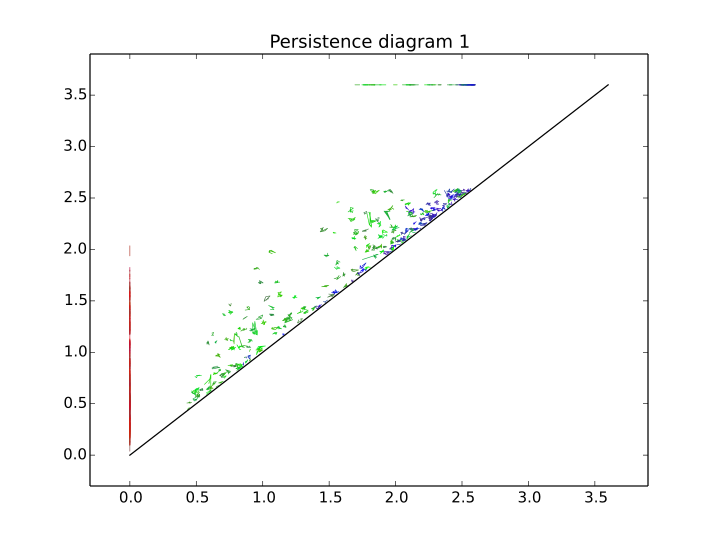
\includegraphics[width=1.2\textwidth]{data3_d2_6_pers.png}
   \caption{Persistance diagram for original and shaken dataset 3}
   \label{data3_pers}
\end{figure}

\begin{figure}[H]
   \centerfloat
   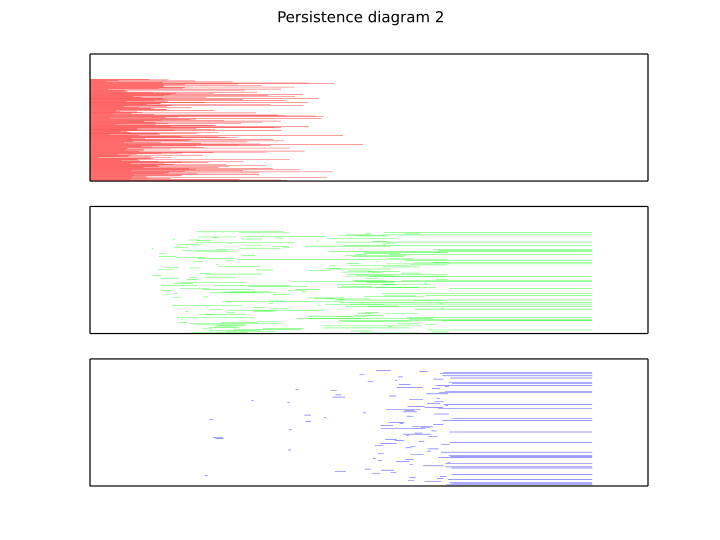
\includegraphics[width=1.2\textwidth]{data3_d2_6_bar.png}
   \caption{Barcode diagram for original and shaken dataset 3}
   \label{data3_bar}
\end{figure}

\end{document}
